% !TEX root = ../../../main/aws_chabauty.tex
\newpage
\subsection{Lecture 3}

Let $p$ be any prime number. Let $X$ be a smooth, $\Z_p$-scheme of relative dimension $d$. Let $x \in X(\F_p)$. 
	\[
	\begin{tikzcd}
	X(\Z_p) \arrow[draw=none]{d}[sloped,auto=false]{\subseteq} \arrow{r} & X(\F_p) \arrow[draw=none]{d}[sloped,auto=false]{\subseteq} \\
	X(\Z_p)_n \arrow{r} & \{n\}
	\end{tikzcd}
	\]
Let $p, t_1,\ldots,t_d$ be generators of the maximal ideal in $\O_{X,n}$.
	\[
	\begin{tikzcd}
	X(\Z_p) \arrow{r}{??} \arrow[bend right=50]{rr}{\Z:= (\Z_1,\ldots,\Z_d)= (t_1,p,t_2/p,\ldots,t_d/p} & p\Z_p^d \arrow{r}{\phi,\sim} & \Z_p^d
	\end{tikzcd}
	\]

Geometrically, shrink $X$ such that it is affine, $t$ regular, and 
	\[
	\begin{tikzcd}
	t^\et: X \arrow{r} & \A^d_{\Z_p} & \Z_p[t_1,\ldots,t_d] \arrow{dd}{t_i \to p \tilde{t}_i} \arrow[dash]{l} \\
	\tilde{X}_x^L \arrow{r} \arrow{u}{\pi} \arrow[draw=none]{d}[sloped,auto=false]{\subseteq} & \A^d_{\Z_p^n} \arrow{u} & \\
	\tilde{X}_x^p \arrow{r} & \A^d_{\Z_p} \arrow[bend right=50,two heads]{uu}{p}  \arrow{u} & \Z_p[\tilde{t}_1,\ldots,\tilde{t}_n]
	\end{tikzcd}
	\]
is the blow up in $x$. Note $t^{-1}(\F_p)= \{x\}$ and $\tilde{t}_i= t_i/p$. Now a picture for the case $d=1$ and $p=5$.


	\begin{figure}[!ht]
	\centering
	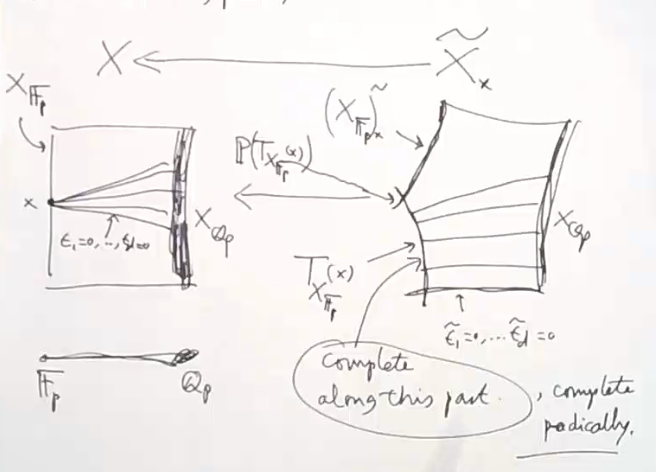
\includegraphics[width=0.5\textwidth]{../images/im31.png}
	\end{figure}

This gives $\Z_p\langle \tilde{t}_1,\ldots,\tilde{t}_d \rangle= \Z_p[ \tilde{t}_1,\ldots,\tilde{t}_d]^{\vee p}$ is $p$-adically complete. 


$\ov{\F}_p \otimes_{\Z_p} (\O(\tilde{X}_x^p)^{\vee p})= \F_p[\tilde{t}_1,\ldots,\tilde{t}_d]$ germ $T_{X_{\F_p}}(x)$. 


On Theorem 4.12 



	\begin{figure}[!ht]
	\centering
	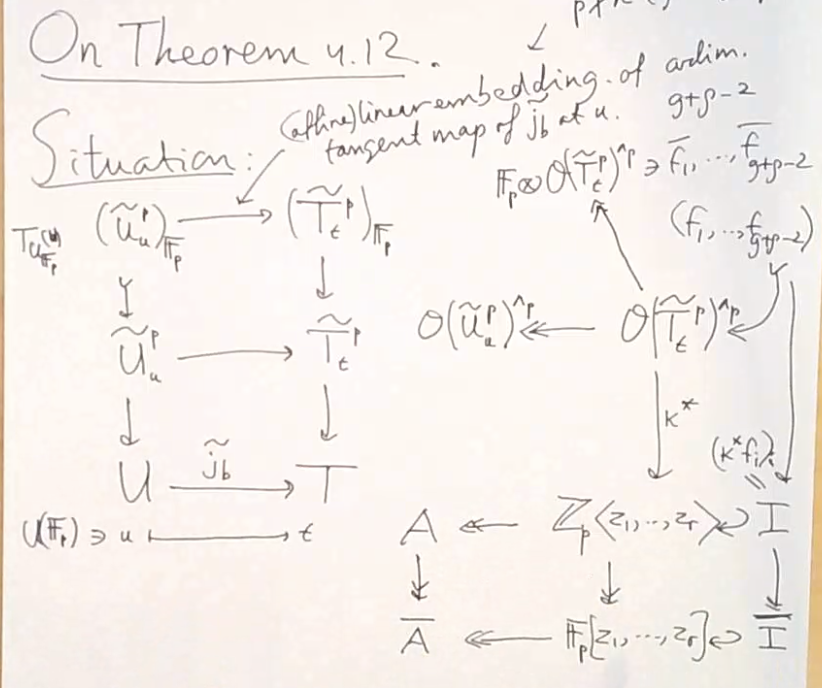
\includegraphics[width=0.5\textwidth]{../images/im32.png}
	\end{figure}

	\begin{figure}[!ht]
	\centering
	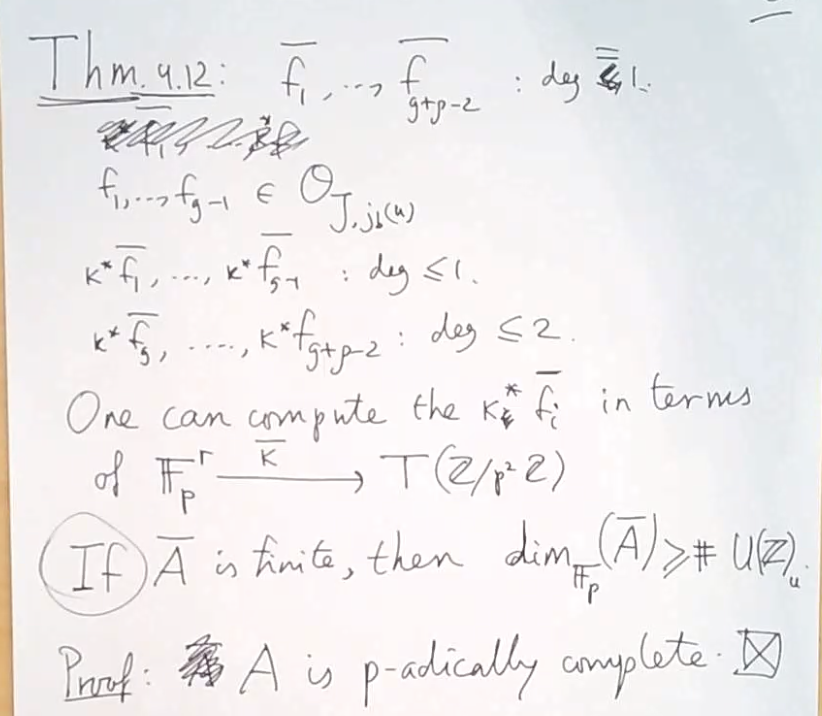
\includegraphics[width=0.5\textwidth]{../images/im33.png}
	\end{figure}


























